\section{Medidas de Forma}
\subsection{Coeficientes de Asimetría}
\begin{itemize}
\item \textbf{Primer Coeficiente de Pearson} $(S_p)$
$$S_p=\dfrac{\overline{x}-M_o}{S} \hspace{1cm} \textrm{en distribuciones Unimodales}$$
\item \textbf{Segundo Coeficiente de Pearson} $(S_p)$
$$S_p=\dfrac{3(\overline{x}-M_e)}{S}$$
\item \textbf{Coeficiente de Asimetría de Bowley} $(S_q)$
$$S_q=\dfrac{(Q_3-M_e)-(M_e-Q_1)}{Q_3-Q_1}=\dfrac{Q_3-2Q_2+Q_1}{Q_3-Q_1}$$
\item \textbf{Coeficiente de Asimetria de Fisher} $(S_m)$
$$S_m = \dfrac{M_3}{\sqrt{M_2^3}}$$
\end{itemize}
\subsection{Curtosis o Apuntalamiento}
Se entiende como el grado de deformación vertical a la curva de frecuencia, con relación al grado de apuntalamiento tenemos:
\begin{center}
\begin{tikzpicture}
\begin{axis}[
  every axis plot post/.append style={mark=none,domain=-8:8,samples=50,smooth}, 
  hide axis,
  legend style={at={(0.5,-0.1)},anchor=north}
  ] 
 \addplot[blue, ultra thick] {gauss(0, 1.25)};
 \addplot[black, ultra thick] {gauss(0, 6)};
 \addplot[red, ultra thick] {gauss(0, 3)};
 
\addlegendentry{Leptocúrtica}
\addlegendentry{Platicúrtica}
\addlegendentry{Mesocúrtica}
\end{axis}
\end{tikzpicture}
\end{center}
\subsubsection{Curtosis en función del Momento}
$$a_4=\dfrac{M_4}{S^4}=\dfrac{M_4}{M_2^2}$$
\subsubsection{Interpretación}
\begin{itemize}
\item $a_4=3\Rightarrow$ la Curva es Mesocúrtica.
\item $a_4>3\Rightarrow$ la Curva es Leptocúrtica.
\item $a_4<3\Rightarrow$ la Curva es Platicúrtica.
\end{itemize}
\section{Medidas de Concentración}
Las medidas de concentración sirven para estimar el grado de igualdad en el reparto o grado de desigualdad de la distribución de cantidades económicas, riquezas, sueldos, etc. También sirve para analizar la concentración poblacional de un terriorio.
\subsection{Indice de Gini $(G)$}
Mide el grado de concentración a través de la diferencia entre $p_i$ y $q_i$ correspondientes, donde $p_i$ y $q_i$ son porcentajes acumulados de la distribución.\\${ }$\\La sumatoria es desde $i=1$ a $k-1$ porque resultaría en cero.
\subsubsection{Cálculo}
$$G=\dfrac{\displaystyle\sum_{i=1}^{k-1}(p_i-q_i)}{\displaystyle\sum_{i=1}^{k-1}p_i}$$
Observar que $0\leq G \leq 1$ y $0\leq\frac{G}{2}\leq \frac{1}{2}$.
\subsubsection{Interpretación de $\frac{G}{2}$}
Si $\frac{G}{2}>10\%$ se considera que la distribución es alta.
\subsection{Curva de Lorenz}
\begin{center}
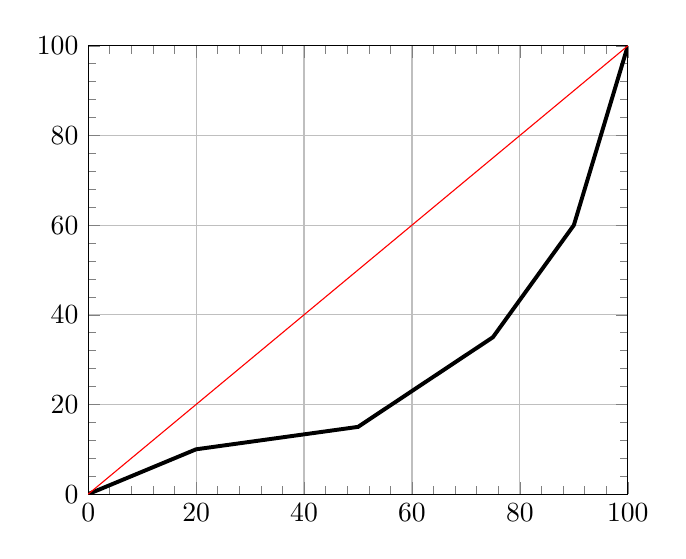
\begin{tikzpicture}
\begin{axis}[
    xmin=0, xmax=100,
    ymin=0, ymax=100,
    minor tick num = 4,
    grid,
    ]
\addplot[color=black,line width=0.5mm] plot 
    coordinates { (0,0) (20,10) (50,15) (75,35) (90,60) (100,100)};
\addplot[color=red] plot
    coordinates { (0,0) (100,100)};
    

\end{axis}
\end{tikzpicture}
\end{center}
